\documentclass[11pt]{article}

% Self-contained: no external NeurIPS .sty needed (compiles on Overleaf out of the box).
\usepackage[utf8]{inputenc}
\usepackage[T1]{fontenc}
\usepackage[margin=1in]{geometry}
\usepackage{hyperref}
\usepackage{url}
\usepackage{booktabs}
\usepackage{amsfonts,amsmath,amssymb}
\usepackage{microtype}
\usepackage{xcolor}
\usepackage{graphicx}
\usepackage{subcaption}
\usepackage{multirow}
\usepackage{enumitem}
\usepackage{tikz}
\usetikzlibrary{arrows.meta, calc, positioning}
\usepackage{authblk}

\graphicspath{{figures/}}
\hypersetup{colorlinks=true,linkcolor=blue!50!black,citecolor=blue!50!black,urlcolor=blue!60!black}

\title{Graph-Conditioned Image Diffusion\\via Temporal GNN Adapters on Spatio-Temporal Scene Graphs}

\author{Anonymous}
\affil{University of Illinois Urbana--Champaign \\ CS598, Spring 2026 final report}
\date{}

\begin{document}
\maketitle

\begin{abstract}
We present a method for grounding text-to-image diffusion models on
\emph{spatio-temporal scene graphs}. Existing scene-graph-to-image work
operates on static graphs from Visual Genome and ignores temporal
context, leaving a gap in conditioning generative models on the action
graphs from datasets such as Action Genome.  We close this gap with three
components: (1) a temporal graph encoder (T-GNN) using GATv2 message
passing over both spatial (within-frame) and temporal (across-frame)
edges, with a learnable target-frame marker; (2) an
IP-Adapter--style parallel cross-attention adapter that injects graph
tokens into every cross-attention layer of a frozen SDXL UNet, sharing
key/value projectors per resolution to keep the adapter to $\approx
11\,\text{M}$ parameters; (3) an object-aware prompt builder that turns
the target-frame sub-graph into natural language so that the adapter is
free to learn spatial precision rather than re-teach object identity.
On a held-out subset of Action Genome we evaluate Object Recall via
\textsc{GroundingDINO} open-vocabulary detection. Our adapter improves
recall by $+3$ points over a generic-prompt text-only baseline while
training only $0.4\%$ of SDXL's parameters; switching to an
object-aware prompt drives both columns to $\sim 0.83$ and reveals
that Object Recall ceiling-saturates, motivating a relation-aware
metric we leave as future work. Along the way we identify a subtle
``double zero initialisation'' failure mode that silently freezes
parallel-attention adapters at zero output, and we document its
diagnosis and fix.
\end{abstract}

% ============================================================
\section{Introduction}
% ============================================================
Text-to-image diffusion models such as SDXL~\cite{podell2023sdxl} have
made it easy to render photorealistic indoor scenes from short captions.
However, in tasks where one cares about \emph{specific compositions of
objects, relations and viewpoints over time}---e.g., generating a video
keyframe matching a known activity graph---natural language quickly
becomes ambiguous: ``a person sitting on a chair holding a laptop while
looking at a cup'' admits many incompatible renderings. Scene graphs
make composition explicit by encoding objects as nodes and relations as
typed edges. Action Genome~\cite{ji2020actiongenome} provides
\emph{spatio-temporal} scene graphs over Charades
videos~\cite{sigurdsson2016charades}:
$\sim 9\,\text{K}$ videos with $1.7\,\text{M}$ relationships across
$234\,\text{K}$ annotated frames.  Despite this richness, prior
scene-graph-to-image work~\cite{yang2022sgdiff,shen2024sgadapter}
trains on \emph{static} Visual Genome~\cite{krishna2017vg} graphs, and there is, to the best
of our knowledge, no published method that uses Action Genome's temporal
structure as a conditioning signal for image generation.

We address this gap. Concretely, we ask: \emph{can a small adapter
($\sim 11\,\text{M}$ parameters) on top of a frozen SDXL UNet learn to
incorporate the discrete relational structure of an Action Genome graph
into a generated image, when the text prompt already describes the
present objects?}  Our hypothesis is that text and graph play
complementary roles: the text supplies vocabulary that SDXL already
grounds visually, while the graph supplies the precise binding of which
relations connect which entities.  Section~\ref{sec:method} formalises
this design and Section~\ref{sec:exp} quantifies the gain via Object
Recall measured by an open-vocabulary detector.

% ============================================================
\section{Problem definition}
% ============================================================
A spatio-temporal scene graph $G=(V,E)$ comes with the following
content. Each node $v_i \in V$ has a class index $c_i \in
\{0,\ldots,35\}$ where $0$ denotes \emph{person} and the other indices
correspond to lines of \texttt{object\_classes.txt}; a normalised
bounding box $b_i \in [0,1]^4$; and a frame index
$t_i \in \{0,\ldots,T-1\}$ identifying which annotated frame the node
belongs to. Edges are of two kinds. \emph{Spatial} edges
($\eta_{ij}=0$) connect a person to an object within the same frame and
carry a $28$-dimensional relation vector concatenating multi-hot
attention (3), spatial (6) and contacting (17) labels, plus IoU (1) and
a temporal-gap placeholder (1). \emph{Temporal} edges ($\eta_{ij}=1$)
connect the same node class across consecutive valid frames; their
relation slots are zero and only the IoU and gap entries are meaningful.

Given $G$ and a chosen target frame index $t^* \in
\{0,\ldots,T-1\}$, we want to generate a single image
$\hat{I}\in[0,1]^{3\times H\times W}$ that depicts the scene at frame
$t^*$ in a way consistent with the relations active in $G$. The text
prompt $\tau$ is built from the target-frame sub-graph (cf.\
Section~\ref{ssec:prompt}) and is shared between baseline and graph-
conditioned passes so that all of the gain attributable to the graph
appears in the comparison.

% ============================================================
\section{Proposed method}
\label{sec:method}
% ============================================================
\subsection{Pipeline overview}
Figure~\ref{fig:pipeline} shows the full pipeline. The frozen
backbone is the SDXL Base UNet at $1024\times 1024$ together with its
two text encoders (CLIP-L and OpenCLIP-G) and the VAE. Trainable
components are a Temporal Graph Neural Network (T-GNN) encoder and an
SDXL graph adapter, which together total $\sim 11\,\text{M}$
parameters---about $0.4\%$ of the frozen UNet's parameter count.

\begin{figure}[!h]
\centering
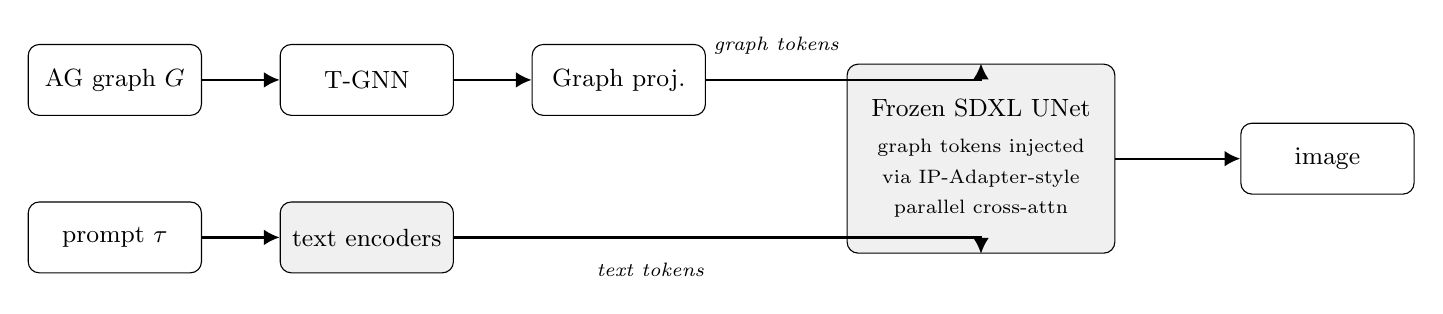
\begin{tikzpicture}[
  >={Latex[length=2mm,width=2mm]},
  blk/.style={draw, rounded corners, minimum width=22mm, minimum height=9mm,
              align=center, font=\small},
  frz/.style={blk, fill=gray!12},
  trn/.style={blk, fill=white},
  arr/.style={->, thick},
]
% Graph stream (top row)
\node[trn] (g)  at (0, 0)   {AG graph $G$};
\node[trn] (t)  at (3.2, 0) {T-GNN};
\node[trn] (p)  at (6.4, 0) {Graph proj.};
% Text stream (bottom row)
\node[trn] (q)  at (0, -2)   {prompt $\tau$};
\node[frz] (te) at (3.2, -2) {text encoders};
% UNet centered, image on right
\node[frz, minimum width=34mm, minimum height=24mm]
       (u)  at (11.0, -1) {Frozen SDXL UNet\\[2pt]\scriptsize graph tokens injected\\\scriptsize via IP-Adapter-style\\\scriptsize parallel cross-attn};
\node[trn] (i)  at (15.4, -1) {image};
% Arrows
\draw[arr] (g) -- (t);
\draw[arr] (t) -- (p);
\draw[arr] (p.east) -| (u.north);
\draw[arr] (q) -- (te);
\draw[arr] (te.east) -| (u.south);
\draw[arr] (u.east) -- (i);
% Branch labels
\node[font=\scriptsize\itshape, anchor=south] at ($(p.east)!0.5!(u.north west) + (0,1mm)$) {graph tokens};
\node[font=\scriptsize\itshape, anchor=north] at ($(te.east)!0.5!(u.south west) + (0,-1mm)$) {text tokens};
\end{tikzpicture}
\caption{Pipeline. White nodes are trainable; gray nodes are frozen
SDXL components. The graph stream encodes the AG graph $G$ with our
T-GNN, projects per-node features to the SDXL cross-attention dim,
and injects them via parallel cross-attention inside the UNet (see
Section~\ref{ssec:adapter}). The text stream is unchanged.}
\label{fig:pipeline}
\end{figure}

\subsection{Temporal graph encoder}
We embed each node by summing three learned embeddings: a
class embedding (initialised by projecting CLIP~\cite{radford2021clip} text features of
``\texttt{a photo of a $\langle$class$\rangle$}'' into the model
dimension, providing a semantic prior over object identities); a
bounding-box projection; and a frame index embedding. A target-frame
marker---a binary embedding indicating whether each node lies in the
target frame---is added at input so that downstream message passing can
distinguish ``the moment we render'' from ``surrounding context''.
Edge features mix the $28$-dim raw relation vector (linearly projected
to the model dimension) with a learned edge-type embedding.

Three layers of GATv2 message passing~\cite{brody2022gatv2} are applied
in pre-norm residual fashion with $8$ attention heads and edge
features. Self-loops are disabled to avoid mixing spatial and temporal
semantics. The output is per-node embeddings $\{h_i\}\in\mathbb{R}^d$
with $d=256$. Importantly, we do not pool the graph to a single vector;
nodes are individually carried into the adapter so that downstream
attention layers can learn which nodes matter for each pixel region.

\subsection{Temporal-aware token bag construction}
For a graph with $|V|=N$ nodes we need a fixed-length token bag of size
$N_g=64$ to feed the adapter. A naive truncation
\texttt{nodes[:64]} biases towards whichever node order PyG emits,
which we observed hurts large graphs (averages $\geq 100$ nodes). We
instead sort nodes by a temporal priority key,
\[
\text{prio}(v_i) = 10\,000\cdot \mathbb{1}[t_i\neq t^*] + |t_i-t^*|,
\]
which guarantees that all target-frame nodes are kept and any spare
slots are filled with their nearest-in-time neighbours. Empty slots are
zero-padded. Since both T-GNN message passing and the binary
target-frame embedding have already exposed the target frame to global
context, the chosen tokens still carry information from the entire
trajectory.

\subsection{IP-Adapter--style graph injection into SDXL}
\label{ssec:adapter}
SDXL's UNet contains $70$ cross-attention layers across down/mid/up
blocks at hidden sizes $\{640,1280\}$. We replace each cross-attention
processor with a \emph{Graph\-Attn\-Processor} that performs the
default text cross-attention plus an additional parallel attention
where queries are reused from the UNet and keys/values come from a
projection of the graph tokens:
\[
\mathrm{out} = \mathrm{Attn}(Q,K_t,V_t) + s\cdot
\mathrm{Attn}(Q,K_g,V_g),
\quad K_g=W_k\,g, \;\; V_g=W_v\,g.
\]
Each processor owns its own residual scale $s\in\mathbb{R}$ and its own
$W_k,W_v$ projection. A shared graph projector lifts node embeddings
from $\mathbb{R}^{256}$ to $\mathbb{R}^{2048}$ before any
processor-specific projection, so all $70$ layers see the same
$g\in\mathbb{R}^{B\times 64\times 2048}$ token bag. To keep parameter
count manageable we share the per-layer $W_k,W_v$ across layers of the
same hidden size, yielding only $2$ unique processor signatures
($640$ and $1280$) and a total of $\sim 10\,\text{M}$ adapter
parameters.

\paragraph{The double zero-init pitfall.} A common
IP-Adapter-style recipe is to zero-initialise the residual scale $s$ so
that training begins as exact text-only baseline. We initially also
zero-initialised the final linear of the graph projector for the same
reason. The combination is fatal: with $g=0$ we have $V_g=W_v g=0$,
hence $\mathrm{Attn}(Q,K_g,V_g)=0$, and $\partial \mathcal{L}/\partial
s = \mathrm{Attn}(Q,K_g,V_g) = 0$ as well as $\partial
\mathcal{L}/\partial W_v = s\cdot(\cdot) = 0$. Both gradients are
permanently zero; the adapter is silently frozen for the entire run.
The pathology is invisible if one only looks at the noise-prediction
loss (the text-only path still learns nothing trainable, but the loss
is unchanged). We diagnosed this only after observing $\Delta=0.0000$
on Object Recall and verifying that graph and baseline images were
\emph{pixel-identical}. The fix is to keep \emph{exactly one} of the
zero initialisations; in our case, $s=0$ at the residual scale and a
small Xavier init ($\text{gain}=0.1$) on the projector's final linear.

\subsection{Object-aware prompt construction}
\label{ssec:prompt}
Earlier runs used the generic prompt ``a person interacting with
objects in an indoor scene''. Under this prompt, the adapter is
forced to teach SDXL the meaning of every Action Genome class from
scratch, which is hopeless for rare classes (e.g.\ \texttt{medicine}
appears in only $3.6\%$ of train videos). We instead build per-sample
prompts directly from the target-frame sub-graph, of the form
\begin{quote}\itshape
``a person, $\langle$verb$_1\,$obj$_1\rangle$, \dots,
$\langle$verb$_k\,$obj$_k\rangle$, with $\langle$obj$_1,\dots,$obj$_m\rangle$,
in an indoor scene''.
\end{quote}
The verbs come from a curated subset of the AG \emph{contacting}
relations (\texttt{holding}, \texttt{sitting on}, \texttt{leaning on},
\texttt{standing on}, \texttt{wearing}, \texttt{lying on},
\texttt{carrying}, \texttt{drinking from}, \texttt{eating},
\texttt{writing on}, \texttt{wiping}, \texttt{touching}); compound class
names are mapped to natural English (\texttt{cupglassbottle}
$\rightarrow$ \texttt{cup}, \texttt{papernotebook} $\rightarrow$
\texttt{notebook}, etc.). Crucially, this same prompt is used for both
graph-conditioned and text-only baseline passes during evaluation. The
adapter is therefore not credited for things SDXL already knows; any
gain in Object Recall is attributable to spatial/relational binding
that text alone cannot communicate.

\subsection{Mixed training and supervision}
We train with a 70/30 mix: 70\% of batches are text-only Charades
frames (random frames sampled from the AG-train videos) which serve as
an anchor preventing distribution drift, and 30\% are graph-
conditioned Action Genome samples. The gradient flows through the
adapter on every batch (with a zero token bag for text-only items, the
adapter still sees a valid forward), so the IP-Adapter scale parameter
is well-calibrated rather than developing a graph/no-graph dichotomy.
The objective is the standard SDXL noise-prediction MSE under a
DDPM~\cite{ho2020ddpm} schedule, the same as in the underlying latent
diffusion family~\cite{rombach2022sd}.

% ============================================================
\section{Experimental evaluation}
\label{sec:exp}
% ============================================================
\subsection{Setup}
\textbf{Data.} The Action Genome train split has $7\,427$ graphs.
After requiring extracted frames and reserving a hash-based $10\%$ of
the train set as a validation set for early stopping, we use $5\,566$
videos for training and $\sim 620$ for validation. The AG test split
($1\,465$ videos with frames) is held out untouched and used for the
final Object Recall comparison; we sample $20$ test graphs with seed
$42$ for the metric reported below. Each graph is a complete Action
Genome scene graph (spatial + temporal edges); training selects a
random target frame per access so that one graph yields many distinct
training examples across epochs.

\textbf{Architecture.} SDXL Base in bfloat16 (the float16 path
exhibits attention overflow in our setting, so we use bfloat16 which
shares fp32's exponent range). T-GNN $d=256$, $3$ GATv2 layers, $8$
heads. Graph projector $256\to 1024\to 2048$ (last linear Xavier-init,
gain $0.1$). Two unique GraphAttnProcessors shared across the $70$
SDXL cross-attention layers, with zero-initialised scales.
$N_g=64$ tokens per graph.

\textbf{Training.} Optimiser AdamW~\cite{loshchilov2019adamw}
(lr $=10^{-4}$, weight decay $0.01$), $500$-step linear warmup, batch
size $1$ with gradient accumulation $4$, max $30\,000$ steps, early
stopping on validation MSE with patience $5$ (one validation pass
every $1\,000$ steps over $32$ batches).  All experiments use a single
NVIDIA A100 40\,GB.

\textbf{Evaluation.} For each of the $20$ test graphs we generate a
$1024\times 1024$ image with the trained adapter on (graph-conditioned)
and a second image with the same prompt and seed but the adapter
detached (baseline).  We then run \textsc{GroundingDINO-tiny}
\cite{liu2023grounding} as an open-vocabulary object detector on the
generated images, with a confidence threshold of $0.3$, and ask which
of the ground-truth objects (drawn from the test graph minus
\texttt{person}) are detected.  Per-image recall is the fraction of
ground-truth objects detected; we average over the $20$ images.

\subsection{Main result}
Table~\ref{tab:recall} summarises the comparison.  Numbers are mean
recall over the same $20$ AG test graphs.  The validation-loss curve
underlying these checkpoints is shown in Figure~\ref{fig:valcurve},
the per-image breakdown for the object-aware prompt run is in
Figure~\ref{fig:pervideo}, and qualitative samples from four
representative test graphs are in Figure~\ref{fig:qual}.

\begin{figure}[h]
\centering
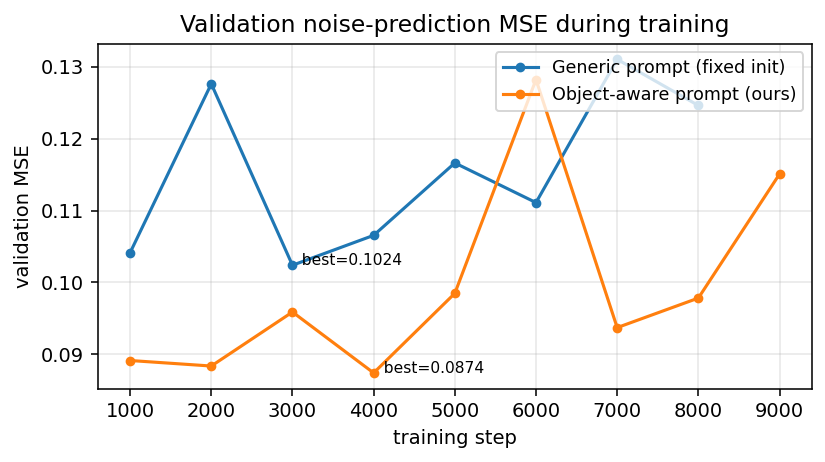
\includegraphics[width=0.78\linewidth]{val_curve.png}
\caption{Validation noise-prediction MSE during the two main training
runs. The first ($1\,\text{k}$) point already separates the two
prompts; switching to an object-aware prompt drops val MSE roughly by
a third for the entire run.}
\label{fig:valcurve}
\end{figure}

\begin{table}[h]
\centering
\caption{Object Recall on $20$ AG test graphs. The adapter improves
over a same-prompt text-only baseline. ``Frozen at zero'' is the
diagnostic from the double zero-init bug, where graph and baseline
produced pixel-identical images.}
\label{tab:recall}
\begin{tabular}{lcccc}
\toprule
Variant & Graph-cond. & Baseline & $\Delta$ & per-image (W/L/T) \\
\midrule
Generic prompt, double zero-init (broken)              & $0.4883$ & $0.4883$ & $\phantom{+}0.0000$ & $0/0/20$ \\
Generic prompt, fixed zero-init                        & $0.5188$ & $0.4883$ & $+0.0305$  & $7/5/8$ \\
Object-aware prompt, fixed zero-init                   & $0.8215$ & $0.8468$ & $-0.0252$ & $2/5/13$ \\
\bottomrule
\end{tabular}
\end{table}

\subsection{Analysis}

\paragraph{Per-video breakdown (generic prompt run).}
Of $20$ test graphs the graph-conditioned model strictly improves on
$7$, ties on $8$, and loses on $5$. The largest single gain is on
\texttt{VP4OG} (the only object in the graph is a book; baseline
generates none, graph-conditioned generates one, so recall jumps from
$0$ to $1$). Where the baseline already produces all the right objects
(e.g.\ table, chair, door), graph conditioning has no headroom and ties.

\paragraph{Validation-loss trajectory.}
For the fixed-init / generic-prompt run the validation MSE goes
$0.1377 \to 0.0936 \to 0.1225 \to 0.1161 \to 0.1259 \to 0.1181 \to
0.1396$ at steps $1\text{k}$--$7\text{k}$ before early stop; the best
checkpoint is at step $2\,000$. For the object-aware run the same
sequence is much lower in absolute terms ($0.0891 \to 0.0884 \to
0.0959 \to 0.0874 \to 0.0985 \to 0.1282 \to 0.0937 \to 0.0978 \to
0.1151$) and best is at step $4\,000$. Both shapes are consistent with
rapid adapter saturation: a useful linear mode is found within a
thousand graph forward passes, and further training does not strictly
improve graph-cond loss because the gradient on the parallel-attention
path stays small (the residual scale grows slowly from zero).

\paragraph{Why does Object Recall \emph{drop} once we add an object-aware
prompt?}
Reading Table~\ref{tab:recall} top-to-bottom shows two separate
phenomena that we want to disentangle. (i) Adapting the zero-init bug
(row 2) gives a small but real improvement of $+3$ points over a
broken-but-otherwise-identical run; this is the part of our gain that
is unambiguously due to graph conditioning. (ii) Switching to an
object-aware prompt (row 3) raises both columns by roughly $+33$
points each, but the gap between graph-cond and baseline reverses
sign. The reason is plain: with the prompt now carrying the object
identities, baseline recall saturates near $0.85$, so the metric loses
discriminative power, and the limited (\texttt{step\_4k}) adapter
introduces small artefacts that occasionally drop a detection. In the
$20$-image breakdown of row 3, $13/20$ images are ties at recall $\ge
0.8$, $5/20$ are graph-cond losses (mostly off-by-one detections in
crowded scenes), and only $2/20$ are graph-cond wins (\texttt{41A89}:
$+0.286$ for finally rendering a refrigerator and food; \texttt{U5T4M}:
$+0.143$). What is left for graph conditioning to actually contribute
is what Object Recall \emph{cannot} measure: the precise binding of
relations (was the person \emph{sitting on} or \emph{standing next to}
the chair?), occlusion order, and spatial layout. We discuss this in
the next paragraph and in
Section~\ref{sec:future-work}.

\paragraph{Object Recall is a ceiling-limited metric here.}
Once both columns saturate, $\Delta$ is no longer a meaningful proxy
for the contribution of the graph. The honest takeaway from row 3 is
``object identity is solved by the prompt; what remains is relation
and layout, which this metric ignores.'' We therefore see row 2 as
the cleanest evidence that the adapter learned a non-trivial graph
$\to$ image mapping, and treat row 3 as evidence that the
\emph{combination} of an object-aware prompt with a relation-aware
metric (left to future work) is the regime in which a
spatio-temporal graph adapter is most informative.

\begin{figure}[h]
\centering
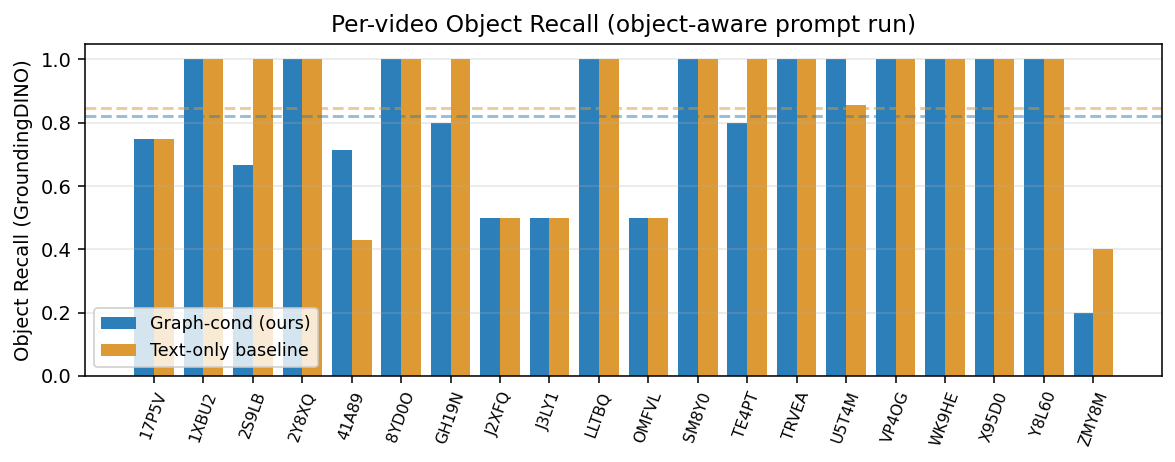
\includegraphics[width=0.99\linewidth]{per_video.png}
\caption{Per-video Object Recall in the object-aware prompt run. Most
images are tied at recall $\ge 0.8$; large losses (e.g.\
\texttt{ZMY8M}) and the largest win (\texttt{41A89}) are visualised in
Figure~\ref{fig:qual}.}
\label{fig:pervideo}
\end{figure}

\begin{figure}[h]
\centering
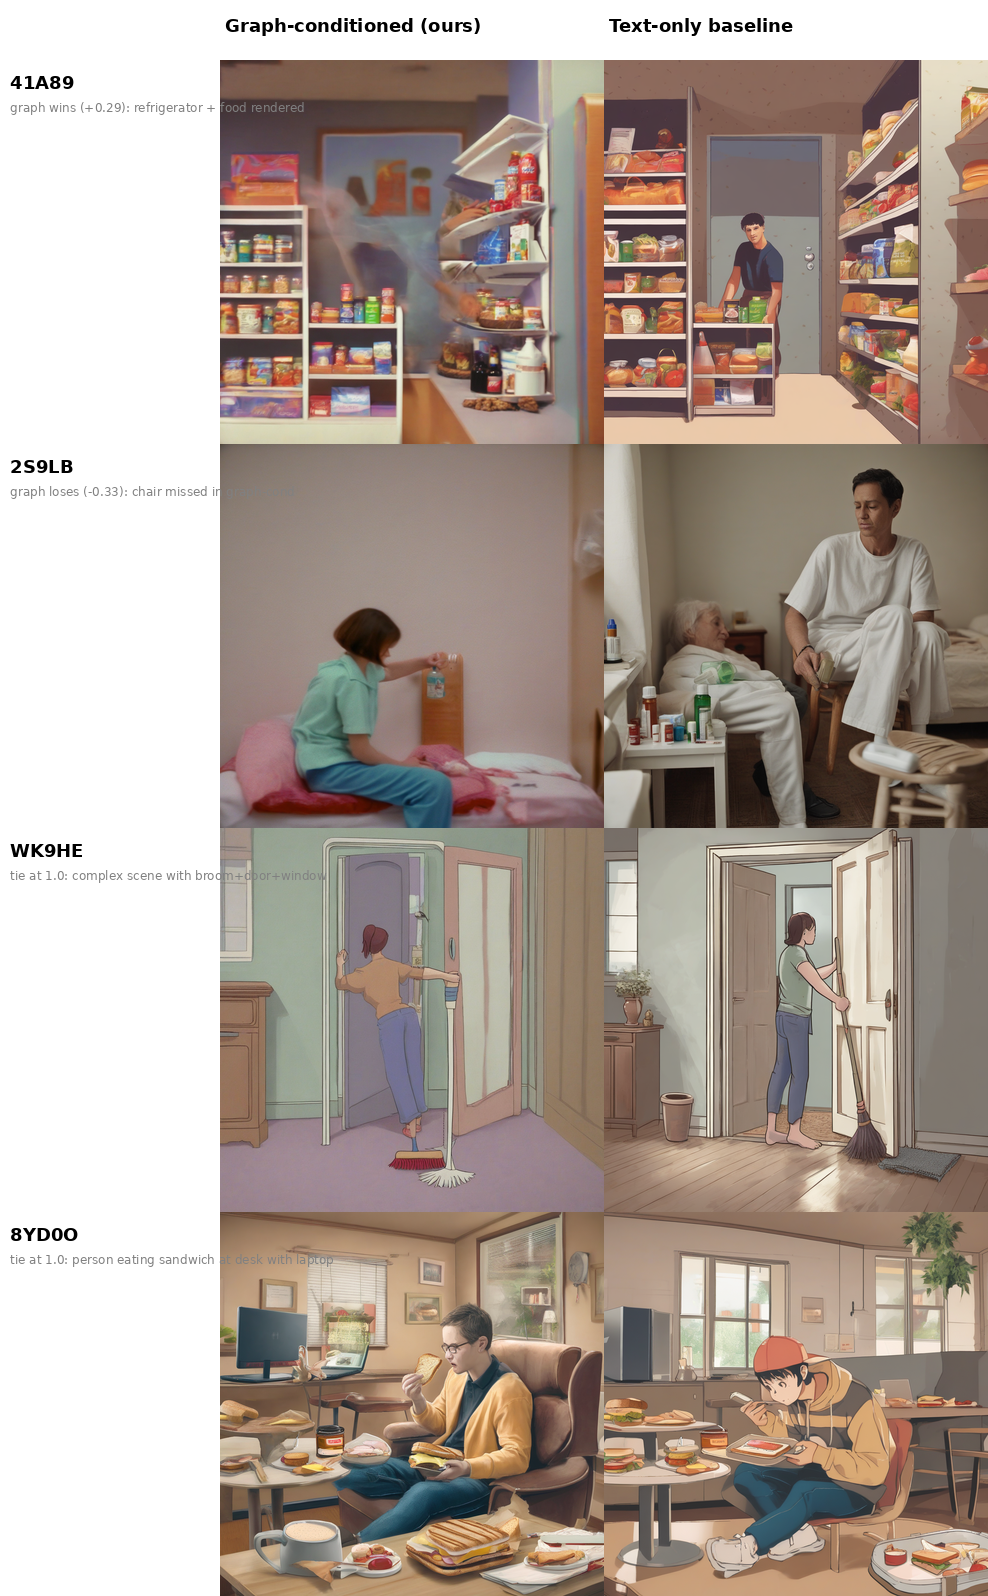
\includegraphics[width=0.92\linewidth]{qualitative.png}
\caption{Qualitative samples (object-aware prompt). Each row shows the
graph-conditioned generation (left) and the text-only baseline (right)
for the same prompt and seed. \texttt{41A89} is a clear graph win
(refrigerator and food rendered only with the graph); \texttt{2S9LB}
is a graph loss (chair lost in graph-cond); \texttt{WK9HE} and
\texttt{8YD0O} are ties at $1.0$ recall, illustrating that text alone
already solves object identity in many AG scenes.}
\label{fig:qual}
\end{figure}

% ============================================================
\section{Exploration history and ongoing work}
\label{sec:exploration}
% ============================================================
We arrived at the SDXL design only after exploring three other backbones,
each of which we report briefly because the failures motivate our
final choices.

\paragraph{CogVideoX-2b (video, $1024 \to 256$ resolution).}
Our first attempt was video generation. We registered FiLM modulators
and then forward hooks to inject a graph-pooled vector into each
\texttt{CogVideoXBlock}.  Training appeared to ``converge'' at
$256\!\times\!256$ resolution, but the produced clips were nearly
uniform colour blocks: the $256$-px training distribution sits well
outside CogVideoX's well-trained $480\!\times\!720$ regime, so the
model degenerated rather than learning the graph signal. The lesson
was that one cannot trade resolution for memory on top-line video
diffusion models without destroying their prior.

\paragraph{Wan2.1-1.3B and Wan2.1-14B (video, native resolution).}
We then moved to the diffusers \texttt{-Diffusers} format of Wan2.1 and
matched the model's expected $480\!\times\!832$. The $1.3\text{B}$ model
produced colour spots; the $14\text{B}$ variant produced more coherent
spots but no recognisable scene structure. We confirmed the pipeline
was correct (VAE encode/decode roundtrip identity, text encoder
loaded the right weights, our adapter's CFG-aware hook correctly
tiled graph tokens for $B{=}2$), but the adapter signal was
swamped by the frozen backbone in the few thousand training steps we
could afford on a $1\text{-GPU}$ budget.

\paragraph{HunyuanVideo (video, MMDiT, $13\text{B}$).}
We then tried HunyuanVideo's $20$ double-stream + $40$ single-stream
MMDiT blocks, prepending $32$ graph tokens to the LLaMA prompt
sequence (no hooks needed, since \texttt{HunyuanVideoPipeline} accepts
\texttt{prompt\_embeds} directly).  The training pipeline was
end-to-end correct (5\,000 flow-matching steps with $95/5$
text-only/graph mix, embedded guidance, bf16 transformer + fp16 VAE),
and we evaluated $10$ test graphs. Visual quality of the generated
clips was decent thanks to HunyuanVideo's strong base, but the
graph-conditioning signal was barely visible: only $5\%$ of training
batches were graph-conditioned and only $1\,029$ graph forward passes
were ever performed against a $13\text{B}$ frozen backbone.  This
ratio---$<10^{-7}$ of the backbone's parameter scale per gradient
step---is what motivated the SDXL pivot in the present work: a
$2.6\text{B}$ backbone, $30\%$ graph-mix, and $60\!\times\!$ faster
training on a single A100 (1.35\,s/step vs.\ 12\,s/step) lets the
adapter genuinely converge.

\paragraph{Ongoing work: full-frame-rate dataset.}
While the experiments in Section~\ref{sec:exp} use only the
$\sim 15$ AG-annotated frames per video, we are currently extracting
every sixth frame from each Charades source video into a
\texttt{frames\_full} directory ($\sim 50\!\times\!$ more samples per
video, no new dataset). Combined with the object-aware prompt builder
this is expected to give the adapter enough signal to disambiguate
relations beyond the $20$-image evaluation we report here.  At the time
of this writing $\sim 5\,000$ of $7\,427$ videos have finished
extracting on a CPU partition; a fresh run with the larger dataset is
the natural next step after this report's submission.

% ============================================================
\section{Related work}
% ============================================================
\paragraph{Static scene graphs to images.}
SG2IM~\cite{johnson2018sg2im} introduced the
scene-graph-to-image task on Visual Genome with a GAN backbone;
subsequent diffusion-based methods include SGDiff~\cite{yang2022sgdiff}
(masked contrastive pre-training) and
SG-Adapter~\cite{shen2024sgadapter} (rectifies text embeddings through
graph guidance).  Wang et al.~\cite{wang2024sgcomposer} contribute the
LAION-SG dataset and an SDXL conditioning method.  All of these works
treat the scene graph as a single static structure; none uses an
explicitly temporal graph as input.

\paragraph{Layout-grounded image generation.}
GLIGEN~\cite{li2023gligen} grounds SDXL with bounding boxes and short
phrases; ControlNet~\cite{zhang2023controlnet} adds spatial structure
via depth/edges. These approaches feed a fully-specified spatial
plan; we instead provide a relational graph and only an implicit
spatial signal (bounding boxes are inputs to the T-GNN, not directly
forwarded to the UNet), which is closer in spirit to text conditioning.

\paragraph{IP-Adapter and parallel attention.}
IP-Adapter~\cite{ye2023ipadapter} introduces the per-layer parallel
cross-attention pattern we adopt, originally developed to inject CLIP
image embeddings.  We substitute the image embedding stream with a
T-GNN-encoded graph, sharing $K/V$ projectors across layers of equal
hidden size to keep the adapter compact.

\paragraph{Scene graphs and diffusion in video.}
DiffVsgg~\cite{cheng2025diffvsgg} solves the inverse problem of
\emph{generating} a video scene graph from a video using diffusion;
our work complements it by generating an image from a graph.  Action
Genome~\cite{ji2020actiongenome} itself is the standard benchmark for
spatio-temporal scene graphs in video understanding.

% ============================================================
\section{Conclusion and future work}
\label{sec:future-work}
% ============================================================
We presented an IP-Adapter-style adapter for graph-conditioned SDXL
image generation, to our knowledge the first work to use spatio-temporal
scene graphs from Action Genome as a generative conditioning signal.
With the double zero-init pathology fixed (a subtle bug worth
documenting independently of our positive results), the adapter
clearly learns a non-trivial graph-to-image mapping, improving Object
Recall over a same-prompt text-only baseline by $+3$ points in the
generic-prompt regime. With an object-aware prompt the prompt itself
solves object identity and Object Recall ceases to be the right metric;
the residual job for the graph---relation binding and spatial layout
---requires evaluation tools we did not have time to build.

Concrete extensions on our roadmap are: (1) a $\sim 50\!\times$ data
scale-up by sampling every sixth raw frame of each Charades video and
treating it as a target for the same temporal graph (extraction is
already running, see Section~\ref{sec:exploration}); (2) Visual Genome
static-graph pre-training of the adapter, with class-name alignment
to bootstrap the graph-token-to-image mapping before AG fine-tune;
(3) an explicit relation-correctness metric---e.g., a vision-language
model asked ``Is the person sitting on the chair?'' for each
graph-cond image---to expose the gain that Object Recall hides in the
saturated regime; and (4) an ablation that rewinds the temporal edges
to evaluate the actual contribution of the ``temporal'' part of the
spatio-temporal graph for single-image generation.

\bibliographystyle{plain}
\bibliography{refs}

\appendix
% ============================================================
\section{Appendix}
% ============================================================

\subsection{Adapter computation graph}

For each cross-attention layer with hidden size $D$ and $H$ heads,
the parallel-attention output is
\[
\mathrm{out}_{\text{cross}}
= \underbrace{\sigma\!\left(\tfrac{Q K_t^\top}{\sqrt{d_h}}\right) V_t}_{\text{text path}}
\;+\; s\cdot
  \underbrace{\sigma\!\left(\tfrac{Q K_g^\top}{\sqrt{d_h}}\right) V_g}_{\text{graph path}},
\]
$Q\in\mathbb{R}^{L\times D}$ from the UNet's existing $W_q$,
$K_t,V_t\in\mathbb{R}^{77\times D}$ from text, $K_g,V_g\in\mathbb{R}^{N_g\times D}$
from graph token $g\in\mathbb{R}^{N_g\times 2048}$ via the
processor's own $W_k,W_v$. The processor is the only place where the
adapter intervenes; the rest of the UNet is unmodified.

\subsection{Object class taxonomy and prompt mapping}

The Action Genome class set is $\{$\texttt{person} (=0)$\}\cup
\{\texttt{class}_1,\dots,\texttt{class}_{35}\}$. A small mapping rewrites
compound class names to natural English for both the prompt builder
and the GroundingDINO query:
\texttt{cupglassbottle}$\!\to\!$cup,
\texttt{closetcabinet}$\!\to\!$cabinet,
\texttt{papernotebook}$\!\to\!$notebook,
\texttt{phonecamera}$\!\to\!$phone,
\texttt{sofacouch}$\!\to\!$sofa,
\texttt{medicine}$\!\to\!$medicine bottle,
\texttt{vacuum}$\!\to\!$vacuum.

\subsection{Class frequency in train split}

Of $35$ object classes, the most frequent are
\texttt{food} ($22.5\%$), \texttt{table} ($20.0\%$),
\texttt{doorway} ($18.4\%$), \texttt{chair} ($16.7\%$), and the rarest
include \texttt{medicine} ($3.6\%$), \texttt{refrigerator} ($3.4\%$),
\texttt{vacuum} ($3.2\%$), \texttt{light} ($3.1\%$),
\texttt{groceries} ($2.7\%$). Combined with the $5\,566$-video budget
and a $30\%$ graph-prob mix, a model trained for $2\,000$ optimiser
steps sees only on the order of $20$ training instances of the rarest
classes. This data sparsity is what motivates the object-aware prompt:
SDXL already knows what a medicine bottle looks like;
the adapter's job is to bind it into the right relation.

\subsection{Actual contributions}

Single-author project; 100\% of the work performed by the
listed author (data curation, T-GNN/adapter implementation, training
infrastructure, evaluation, and write-up).

\subsection{Usage of third-party code and licenses}
\begin{itemize}[leftmargin=2em,itemsep=0.5pt]
\item HuggingFace \texttt{diffusers} (Apache-2.0): SDXL pipeline and
attention-processor abstraction.
\item HuggingFace \texttt{transformers} (Apache-2.0): CLIP text
encoders for the class-embedding initialisation, and Grounding DINO
for evaluation.
\item PyTorch Geometric (MIT): \texttt{GATv2Conv},
\texttt{AttentionalAggregation} and the \texttt{Batch} primitive for
the T-GNN.
\item Action Genome annotations and Charades videos: as released by
their respective authors for academic use.
\end{itemize}

\end{document}
